% Options for packages loaded elsewhere
% Options for packages loaded elsewhere
\PassOptionsToPackage{unicode}{hyperref}
\PassOptionsToPackage{hyphens}{url}
\PassOptionsToPackage{dvipsnames,svgnames,x11names}{xcolor}
%
\documentclass[
  11pt]{article}
\usepackage{xcolor}
\usepackage{amsmath,amssymb}
\setcounter{secnumdepth}{5}
\usepackage{iftex}
\ifPDFTeX
  \usepackage[T1]{fontenc}
  \usepackage[utf8]{inputenc}
  \usepackage{textcomp} % provide euro and other symbols
\else % if luatex or xetex
  \usepackage{unicode-math} % this also loads fontspec
  \defaultfontfeatures{Scale=MatchLowercase}
  \defaultfontfeatures[\rmfamily]{Ligatures=TeX,Scale=1}
\fi
\usepackage{lmodern}
\ifPDFTeX\else
  % xetex/luatex font selection
\fi
% Use upquote if available, for straight quotes in verbatim environments
\IfFileExists{upquote.sty}{\usepackage{upquote}}{}
\IfFileExists{microtype.sty}{% use microtype if available
  \usepackage[]{microtype}
  \UseMicrotypeSet[protrusion]{basicmath} % disable protrusion for tt fonts
}{}
% Make \paragraph and \subparagraph free-standing
\makeatletter
\ifx\paragraph\undefined\else
  \let\oldparagraph\paragraph
  \renewcommand{\paragraph}{
    \@ifstar
      \xxxParagraphStar
      \xxxParagraphNoStar
  }
  \newcommand{\xxxParagraphStar}[1]{\oldparagraph*{#1}\mbox{}}
  \newcommand{\xxxParagraphNoStar}[1]{\oldparagraph{#1}\mbox{}}
\fi
\ifx\subparagraph\undefined\else
  \let\oldsubparagraph\subparagraph
  \renewcommand{\subparagraph}{
    \@ifstar
      \xxxSubParagraphStar
      \xxxSubParagraphNoStar
  }
  \newcommand{\xxxSubParagraphStar}[1]{\oldsubparagraph*{#1}\mbox{}}
  \newcommand{\xxxSubParagraphNoStar}[1]{\oldsubparagraph{#1}\mbox{}}
\fi
\makeatother


\usepackage{longtable,booktabs,array}
\usepackage{calc} % for calculating minipage widths
% Correct order of tables after \paragraph or \subparagraph
\usepackage{etoolbox}
\makeatletter
\patchcmd\longtable{\par}{\if@noskipsec\mbox{}\fi\par}{}{}
\makeatother
% Allow footnotes in longtable head/foot
\IfFileExists{footnotehyper.sty}{\usepackage{footnotehyper}}{\usepackage{footnote}}
\makesavenoteenv{longtable}
\usepackage{graphicx}
\makeatletter
\newsavebox\pandoc@box
\newcommand*\pandocbounded[1]{% scales image to fit in text height/width
  \sbox\pandoc@box{#1}%
  \Gscale@div\@tempa{\textheight}{\dimexpr\ht\pandoc@box+\dp\pandoc@box\relax}%
  \Gscale@div\@tempb{\linewidth}{\wd\pandoc@box}%
  \ifdim\@tempb\p@<\@tempa\p@\let\@tempa\@tempb\fi% select the smaller of both
  \ifdim\@tempa\p@<\p@\scalebox{\@tempa}{\usebox\pandoc@box}%
  \else\usebox{\pandoc@box}%
  \fi%
}
% Set default figure placement to htbp
\def\fps@figure{htbp}
\makeatother





\setlength{\emergencystretch}{3em} % prevent overfull lines

\providecommand{\tightlist}{%
  \setlength{\itemsep}{0pt}\setlength{\parskip}{0pt}}



 
\usepackage[]{natbib}
\bibliographystyle{econ}


\usepackage{graphicx}
\usepackage{bbm}
\usepackage{amssymb}
\usepackage{amsmath}
\usepackage[nomarginpar]{geometry}
\usepackage{setspace}
\usepackage{natbib}
\usepackage{lscape}
\usepackage{rotating}
\usepackage{tabularx, calc}
\usepackage{threeparttable}
\usepackage{picinpar}  
\usepackage{longtable}
\usepackage{ae}
\usepackage{float}
\usepackage{morefloats}
\usepackage{palatino}
\usepackage{hyperref}
\usepackage{color}
\usepackage{adjustbox}
\usepackage{booktabs} 
\usepackage[normalem]{ulem}
\usepackage{ragged2e}
\usepackage{changepage}
\usepackage{longtable}
%\usepackage{graphics}
%\usepackage[tableposition=top]{caption}

\geometry{left=1.0in,right=1.0in,top=1.0in,bottom=1.0in}
\onehalfspacing
\usepackage{booktabs}
\usepackage{longtable}
\usepackage{array}
\usepackage{multirow}
\usepackage{wrapfig}
\usepackage{float}
\usepackage{colortbl}
\usepackage{pdflscape}
\usepackage{tabu}
\usepackage{threeparttable}
\usepackage{threeparttablex}
\usepackage[normalem]{ulem}
\usepackage{makecell}
\usepackage{xcolor}
\newcommand{\mytitle}{High Returns, Low Investment: \\ Public Capital and the Euler Equation Puzzle}
\usepackage{parskip}
\setlength{\parskip}{0.5\baselineskip}
\setlength{\parindent}{2em}
\makeatletter
\@ifpackageloaded{caption}{}{\usepackage{caption}}
\AtBeginDocument{%
\ifdefined\contentsname
  \renewcommand*\contentsname{Table of contents}
\else
  \newcommand\contentsname{Table of contents}
\fi
\ifdefined\listfigurename
  \renewcommand*\listfigurename{List of Figures}
\else
  \newcommand\listfigurename{List of Figures}
\fi
\ifdefined\listtablename
  \renewcommand*\listtablename{List of Tables}
\else
  \newcommand\listtablename{List of Tables}
\fi
\ifdefined\figurename
  \renewcommand*\figurename{Figure}
\else
  \newcommand\figurename{Figure}
\fi
\ifdefined\tablename
  \renewcommand*\tablename{Table}
\else
  \newcommand\tablename{Table}
\fi
}
\@ifpackageloaded{float}{}{\usepackage{float}}
\floatstyle{ruled}
\@ifundefined{c@chapter}{\newfloat{codelisting}{h}{lop}}{\newfloat{codelisting}{h}{lop}[chapter]}
\floatname{codelisting}{Listing}
\newcommand*\listoflistings{\listof{codelisting}{List of Listings}}
\makeatother
\makeatletter
\makeatother
\makeatletter
\@ifpackageloaded{caption}{}{\usepackage{caption}}
\@ifpackageloaded{subcaption}{}{\usepackage{subcaption}}
\makeatother
\usepackage{bookmark}
\IfFileExists{xurl.sty}{\usepackage{xurl}}{} % add URL line breaks if available
\urlstyle{same}
\hypersetup{
  pdfauthor={Yichu Li},
  pdfkeywords={Public Investment, Collective Action, Development
Accounting},
  colorlinks=true,
  linkcolor={red},
  filecolor={Maroon},
  citecolor={red},
  urlcolor={red},
  pdfcreator={LaTeX via pandoc}}


\title{\mytitle}
\author{\LARGE Yichu Li}
\date{March 8, 2026}
\begin{document}
\def\spacingset#1{\renewcommand{\baselinestretch}%
{#1}\small\normalsize} \spacingset{1}


%%%%%%%%%%%%%%%%%%%%%%%%%%%%%%%%%%%%%%%%%%%%%%%%%%%%%%%%%%%%%%%%%%%%%%%%%%%%%%

\date{\href{https://tsssssssshark.github.io/euler-collective-action/output/main.pdf}{Link to Latest version}\\ \vspace{1em}  Last updated March
8, 2026}
\title{\mytitle}
\author{
\LARGE Yichu Li\thanks{The London School of Economics and Political
Science.
\href{mailto:y.li395@lse.ac.uk}{\nolinkurl{y.li395@lse.ac.uk}}.}\\
}
\maketitle

\bigskip
\bigskip
\begin{abstract}
The text of your abstract.
\end{abstract}

\bigskip
\noindent%
{\it Keywords:} Public Investment, Collective Action, Development
Accounting
\vfill

\newpage
\spacingset{1.2} % DON'T change the spacing!

\section{Introduction}\label{sec-intro}

INSERT INTRODUCTION

\section{An Euler Equation Model Incorporating Public
Capitals}\label{sec-model}

I build on the intertemporal optimisation framework of
\citet{kremer2019}. I first consider the case where capital is entirely
public and investment occurs only through taxation, showing that this
generates a collective action problem and a government efficiency
problem that dilutes the effective return to capital when state taxation
capacity and efficiency is low. I then extend this analysis into a
generalised model standard model incorporating both public and private
capital, allowing households to allocate investments between the two.

\subsection{Baseline: Standard Euler Equation}\label{sec-baseline}

Consider in a deterministic discrete-time intertemporal consumption
model, households maximise their discounted lifetime utility over an
infinite time horizon.

\subsubsection*{Optimisation Problem}\label{optimisation-problem}
\addcontentsline{toc}{subsubsection}{Optimisation Problem}

Households face the following optimisation
problem:\begin{equation}\phantomsection\label{eq-optimisation}{
\max_{\{C_t\}} \sum_{t=0}^\infty \delta^t u(C_t)
}\end{equation} where \(0<\delta<1\) is the annual discount factor,
\(C_t\) is the household consumption in period \(t\), and \(u(C_t)\)
measures the utility from consuming \(C_t\) in period \(t\). \(u(C)\) is
increasing and concave and follows Inada Conditions: \(u'(C) > 0\),
\(u''(C) < 0\), \(\lim_{C \to 0} u'(C) = \infty\), and
\(\lim_{C \to \infty} u'(C) = 0\).

\subsubsection*{Budget Constraint}\label{budget-constraint}
\addcontentsline{toc}{subsubsection}{Budget Constraint}

\begin{equation}\phantomsection\label{eq-budget}{
x_{t+1} = f'(K_t)(x_t - C_t)
}\end{equation}\(x_t\) is household assets (`cash on hand') in period
\(t\) with \(x_0\) given, \(C_t\) is consumption in period \(t\), and
\(f'(K_t)\) is the gross return to capital. \(f(K)\) is increasing and
concave, following: \(f'(K) > 0\), \(f''(K) < 0\),
\(\lim_{K \to 0} f'(K) = \infty\), and \(\lim_{K \to \infty} f'(K) = 1\)
(long-run steady state).

\subsubsection*{Discrete Time Euler
Equation}\label{discrete-time-euler-equation}
\addcontentsline{toc}{subsubsection}{Discrete Time Euler Equation}

Solving for optimal intertemporal consumption
path:\begin{equation}\phantomsection\label{eq-euler}{
u'(C_t) = \delta f'(K_t) u'(C_{t+1})
}\end{equation} Assume constant-elasticity-of-substitution (CES)
utility:\[
u(C) = 
\begin{cases}
    \frac{C^{1-\sigma}}{1-\sigma} & \text{if } \sigma \ne 1\\
    \ln(C) & \text{if } \sigma = 1
\end{cases}
\]This means that the elasticity of intertemporal substitution is
constant and independent of \(C_t\). Therefore, the consumption growth
rate is:\begin{equation}\phantomsection\label{eq-growth}{
\frac{C_{t+1}}{C_t} - 1 = (\delta f'(K_t))^{\frac{1}{\sigma}} - 1
}\end{equation}

\subsubsection*{The Puzzle}\label{the-puzzle}
\addcontentsline{toc}{subsubsection}{The Puzzle}

Assume that the model governs the intertemporal consumption behaviour of
a representative household, the model should also apply at a macro
level. To illustrate the puzzle at the macro level, I use
\(\delta = 0.96\)
\footnote{$\frac{1}{\delta} - 1 \approx 0.04$, implying a 4\% annual rate of time preference.}and
\(\sigma = 2\)
\footnote{Elasticity of intertemporal substitution of 0.5 is used in macro studies standard calibrations.}
proposed in \citet{kremer2019}, and internal rates of return from the
Penn World Table (PWT)
\footnote{Available for download at \url{www.ggdc.net/pwt}}
\citep{feenstra2015a} as a proxy for
\(f'(K)\)\footnote{See \url{https://www.rug.nl/ggdc/docs/the_next_generation_of_the_penn_world_table.pdf}}
to model the predicted consumption growth rates under
Equation~\ref{eq-growth}. Intuitively, a concave production function
means that countries with lower capital stock face higher returns on
capital investment. Figure~\ref{fig-k-gdp} shows that countries with
lower income have lower capital stock. Therefore, according to
Equation~\ref{eq-growth}, consumption growth rates should be high.
However, Figure~\ref{fig-actual-predict} Panel (A) shows that in many
middle- and low-income countries, the actual growth rates fall below
what the Euler Equation predicts. Moreover,
Figure~\ref{fig-actual-predict} Panel (B) shows that countries with
higher predicted consumption growth rates tend to have larger gap
between predicted and actual rates. This pattern is most pronounced in
countries such as Egypt, Venezuela, Côte d'Ivoire, and Zimbabwe.
Therefore, the puzzle is why households in these economies invest at
levels far below what the standard model predicts as optimal.

\begin{figure}

\caption{\label{fig-k-gdp}Lower Capital Stock in Lower-Income Countries}

\centering{

\pandocbounded{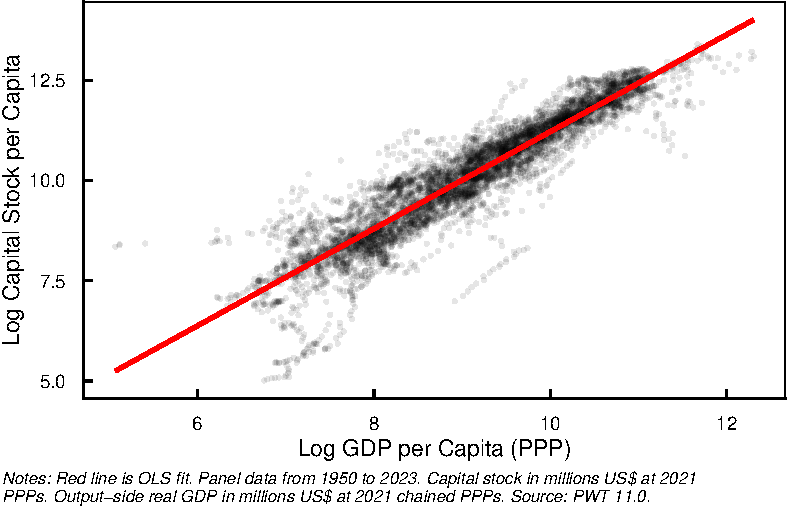
\includegraphics[keepaspectratio]{main_files/figure-pdf/fig-k-gdp-1.pdf}}

}

\end{figure}%

\begin{figure}

\caption{\label{fig-actual-predict}Actual vs.~Predicted Average
Consumption Growth Across Countries 2010-2019}

\centering{

\pandocbounded{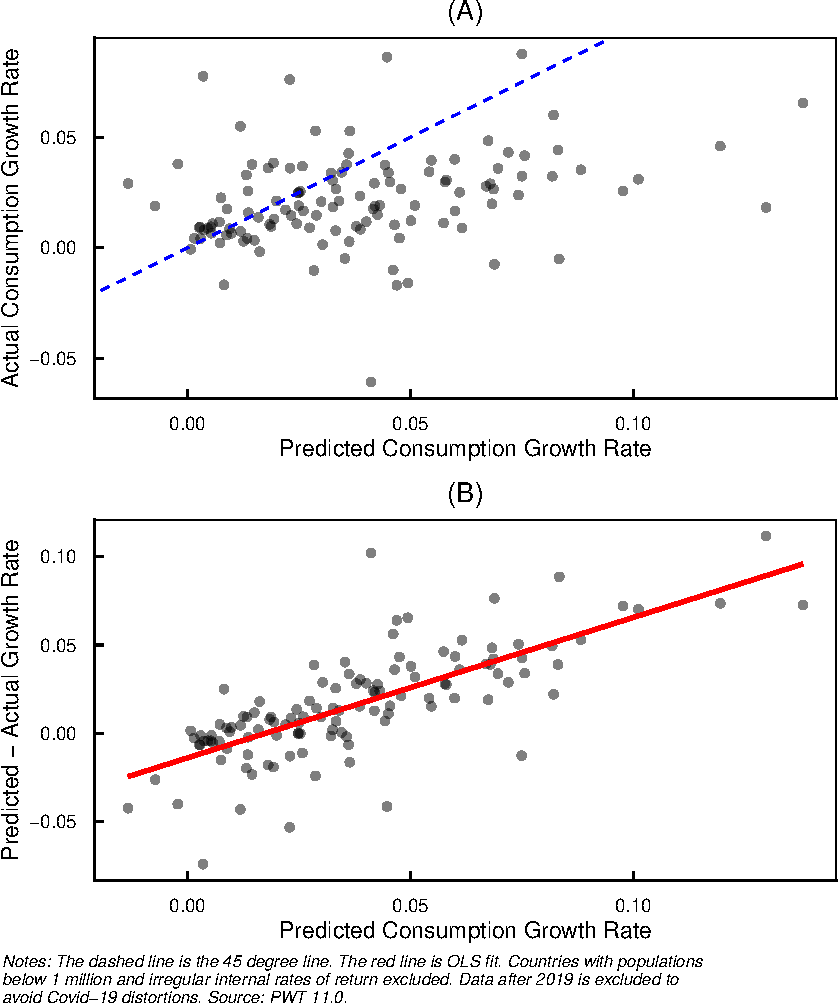
\includegraphics[keepaspectratio]{main_files/figure-pdf/fig-actual-predict-1.pdf}}

}

\end{figure}%

\subsection{Capital as a Public Good}\label{sec-capital-public}

The baseline model in Section~\ref{sec-baseline} assumes capital
investments are private for households. This means that households
receive the full returns \(f'(K)\) because they would own the invested
capital in productions. These are scenarios where farmers invest in
agricultural tools, vendors invest in mobile phones to gather market
information, or freelance drivers invest in a motorcycle or car.
However, capitals with public good features like infrastructure often
require public investment commonly through government spending, and the
benefits from these investments are shared among the population. INSERT
EXAMPLES OF HIGH RETURNS. Since taxes commonly fund the majority of
government spending, households engage with public investment indirectly
through paying taxes. This structure can create a collective action
problem and a government inefficiency problem that produces low levels
of public investments despite high rates of return.

To illustrate this, I will present an extreme case where we assume
capitals are all publicly invested through taxation by governments.
Consider the same optimisation problem as Equation~\ref{eq-optimisation}
with a different budget constraint for homogeneous households in an
economy. For any household \(i\), the budget constraint is:
\begin{equation}\phantomsection\label{eq-budget-public}{
x_{i,t+1} = \frac{1}{N} \cdot \gamma f'(K_t) \cdot [(x_{i,t} - C_{i,t}) + \sum_{\forall j \neq i} (x_{j,t} - C_{j, t})]\
}\end{equation} where \(N\) is the total number of households in the
economy, \(\sum_{\forall j \neq i} (x_{j,t} - C_{j, t})\) is the
aggregate public investment from all other households, and
\(\gamma \in [0,1]\) represents government efficiency. Because public
capitals can only be invested collectively, the total returns depend on
the aggregate investment level, and assume each individual household
receive an equal share of the total returns. Assume the government's
only fiscal spending is on public capital investment, \(\gamma=0\) when
the government effectively invests no tax revenue into public captials
and \(\gamma = 1\) when the government effectively invests all of tax
revenues into public capitals.

\subsubsection*{Weak Taxation Capacity and Government
Efficiency}\label{weak-taxation-capacity-and-government-efficiency}
\addcontentsline{toc}{subsubsection}{Weak Taxation Capacity and
Government Efficiency}

To reflect weak taxation capacity, assume that household \(i\) makes
public investment decision through taxation voluntarily and independent
of other households' decisions. From the perspective of household \(i\),
the total returns from public capital investment as a public good is
diluted among the population. Alternatively, for a fixed level of total
returns on public capital, the impact of the household's investment
level \((x_{i,t} - C_{i,t})\) on its assets in the next period is small
for large \(N\). Weak government efficiency also dilutes the return on
public capitals when \(\lambda\) is small.

Solving for optimal intertemporal consumption path for household \(i\)
given
\(\sum_{\forall j\ne i} (x_{jt} - C_{jt})\):\begin{equation}\phantomsection\label{eq-euler-public}{
u'(C_{i,t}) = \frac{1}{N} \cdot \delta \gamma f'(K_t) u'(C_{i, t+1})
}\end{equation} Notice that when \(N=1\) and \(\gamma = 1\), this
equation is identical to Equation~\ref{eq-euler}, but \(u'(C_{i.t})\)
decreases as \(N\) becomes larger and \(\gamma\) becomes smaller. For
increasing and concave utility function, \(u'(C_{i,t})\) is smaller when
\(C_{i,t}\) is larger. This means that household \(i\) will consume more
and invest less as \(N\) increases and \(\gamma\) decreases. For
sufficiently large \(N\) or sufficently small \(\gamma\) so that the
Euler Equation cannot be satisfied by an interior solution, household
\(i\) will optimally choose a corner solution of consuming all and
invest none. \(\frac{1}{N}\) produces a collective action problem where
the global optimal decision is for all households to invest and benefit
from high \(f'(K)\) but individuals households have a dominant strategy
of not investing. \(\gamma\) produces a problem where fiscal leakages to
corruption or misallocation disincentives the household to invest.

This model captures the reluctant tax compliance in many low- or
middle-income countries where the population is sufficiently large and
the states have weaker taxation capacity and relatively inefficient.
Figure~\ref{fig-tax-gove-gdp} shows these model assumptions are
consistent with the data.

\begin{figure}

\caption{\label{fig-tax-gove-gdp}Higher Tax Revene and Government
Effectiveness in Higher-Income Countries}

\centering{

\pandocbounded{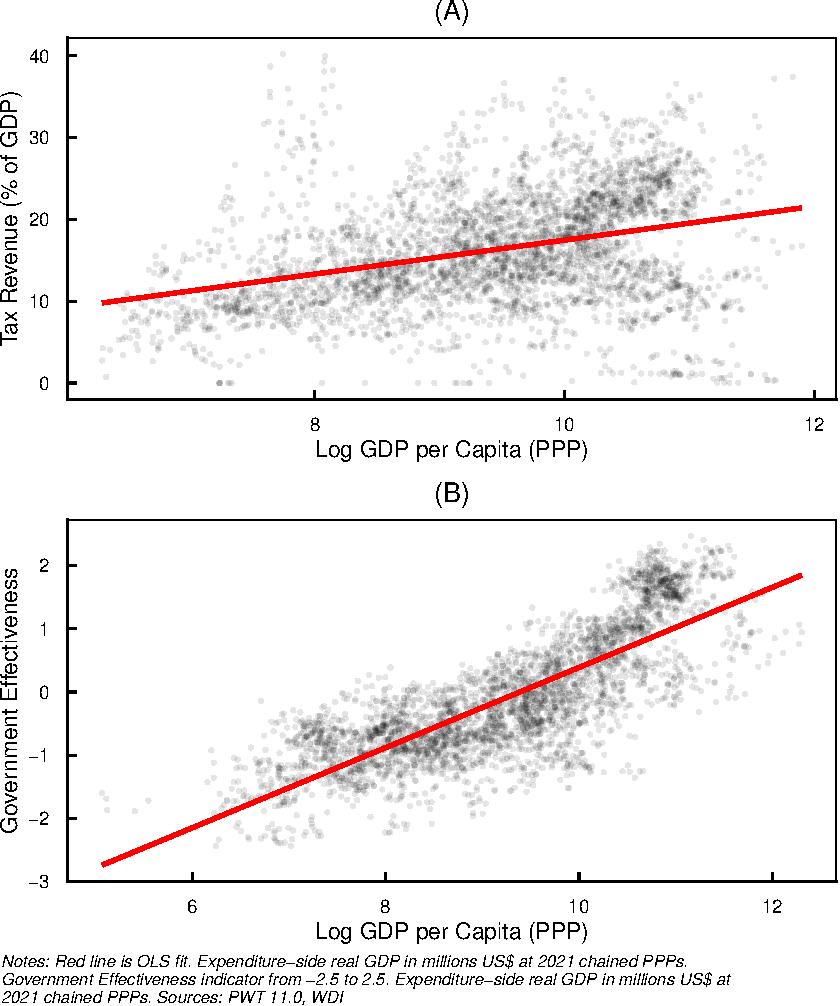
\includegraphics[keepaspectratio]{main_files/figure-pdf/fig-tax-gove-gdp-1.pdf}}

}

\end{figure}%

\subsubsection*{Strong Taxation Capacity and Government
Efficiency}\label{strong-taxation-capacity-and-government-efficiency}
\addcontentsline{toc}{subsubsection}{Strong Taxation Capacity and
Government Efficiency}

Higher income countries tend to have more efficient governments and
stronger taxation capacity because income tax can be more easily
collected from formal employees. Although, public investment is less
voluntary for tax rates as given, households might make public
investment decisions by influencing the tax rates through political
channels. The key difference is that they expect other households to
also comply with the decided upon tax rates.

Consider a simple case of homogeneous households facing the same
optimisation problem as Equation~\ref{eq-optimisation} bu assume perfect
enforcibility upon any chosen taxation level instead and perfect
government efficiency. Any individual household \(i\) chooses a taxation
level (public investment level) \((x_{i,t} - C_{it})\) and expect
symmetry from other households. Because households are homogeneous, the
following should hold: \[
[(x_{i,t} - C_{i,t}) + \sum_{\forall j \neq i} (x_{j,t} - C_{j, t})] = N \cdot (x_{i,t} - C_{i,t})
\]Therefore, the budget constraint becomes identical to
Equation~\ref{eq-budget}: \[
x_{i,t+1} = \frac{1}{N} \cdot 1 \cdot f'(K_t)\cdot N \cdot (x_{i,t} - C_{i,t}) = f'(K_t)(x_{i,t} - C_{i,t})
\] Solving for optimal consumption path will produce an Euler Equation
identical to Equation~\ref{eq-euler}. Note that the collective action
problem is resolved in this setting because the perfect tax enforcement
enables households to optimise consumption conditional on the
expectation of symmetrical behaviours from others.

\subsection*{A Generalised Model}\label{a-generalised-model}
\addcontentsline{toc}{subsection}{A Generalised Model}

In reality, the majority of countries likely fall in between the extreme
cases outlined in Section~\ref{sec-capital-public}. Within a country,
there are likely different extents that households pay taxes, based on
formal or self-employment for example. Therefore, on a macro level, it
depends on whether the collective action problem dominates.

To generalise the model of public investment, I propose the following
budget constraint: \[
x_{t+1} = \frac{1}{N^\lambda} \cdot \gamma f'(K_t^{pub})(x_t - C_t)
\]where \(K_t^{pub}\) is the public capital stock and \(\lambda\) is a
parameter between 0 and 1 that determines the salience of the collective
action problem in public investment. \(\lambda = 1\) if the collective
action problem is most extreme and \(\lambda = 0\) if there is no
collective action problem. Combining this model with the baseline
private capital investment budget constraint gives:
\begin{equation}\phantomsection\label{eq-budget-combined}{
x_{t+1} = r_t^{eff} \cdot (x_t - C_t)
}\end{equation} where \[
r_t^{eff} = (1-PublicShare_t) \cdot f'(K^{priv}_t) + PublicShare_t \cdot \gamma f'(K^{pub}_t)
\] \(K^{priv}\) denoting private capital stock and \(PublicShare\)
denoting the share of public capital investment in total investment. The
returns on private and public capital are derived by this generalised
production function: \[
Y_t = A_t(K_t^{priv})^{\alpha^{priv}}(K_t^{pub})^{\alpha^{pub}}L^{1-\alpha^{priv}-\alpha^{pub}}
\] where the FOCs are:
\begin{equation}\phantomsection\label{eq-returns}{
f'(K_t^{priv}) = \alpha_{priv} \cdot \frac{Y_t}{K_t^{priv}} \quad \text{and} \quad f'(K_t^{pub}) = \alpha_{pub} \cdot \frac{Y_t}{K_t^{pub}}
}\end{equation} Taken all together, solving for optimal consumption path
under constraint given by Equation~\ref{eq-budget-combined} produces an
Euler Equation:
\begin{equation}\phantomsection\label{eq-euler-combined}{
u'(C_t) = \delta \cdot r^{eff} \cdot u'(C_{t+1})
}\end{equation} and consumption growth rate given by:

\begin{equation}\phantomsection\label{eq-growth-combined}{
\frac{C_{t+1}}{C_t} - 1 = (\delta \cdot r^{eff})^{\frac{1}{\sigma}} - 1
}\end{equation}

\section{Stylised Facts}\label{stylised-facts}

\clearpage


\renewcommand\refname{References}
\bibliography{references.bib}



\end{document}
